\documentclass[12pt]{article}

\usepackage{framed}
\usepackage{amsmath}
\usepackage{amssymb}
\usepackage{graphics}
\usepackage{graphicx}
\voffset=-1.5cm
\oddsidemargin=0.0cm
\textwidth = 470pt
\title{Inference Procedures}
%\author{MA4605}
\begin{document}
	
	
\section*{Two-Way Worked Example}

\noindent\textbf{Review Question No 22.} \\

\noindent Three varieties of potatoes are being compared for yield. The experiment
was carried out by assigning each variety at random to four of twelve equal size
plots, one being chosen in each of four locations. The following yields in bushels per 
plot resulted:
% A bushel is about 36.4 litres.

\begin{figure}[h!]
	\centering
	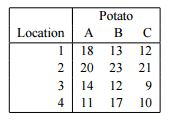
\includegraphics[width=0.4\linewidth]{twowayanova-potato}
\end{figure}
\subsection*{Additional Information} 
\begin{framed}
	\noindent Expect to be given $S^2_R$ and $S^2_C$ in an exam standard question, as well as the variance for the response variable. You will also be given the formula for $\textrm{MS}_{A}$ and $\textrm{MS}_{B}$.\\
	\textit{(\textbf{Important}: Partially Completed table, you would not need this information.)}
\end{framed}

\begin{itemize}
	\item Location is Factor A - it is arranged along the rows
	\item Potato Type is Factor B - it is arranged along the columns.
\end{itemize}
\begin{itemize}
	\item The variance of the Row means is : $S^2_{R} = 19.037$. Therefore 
	\[ \textrm{MS}_{A} = c \times S^2_{R} = 3 \times 19.037 = 57.111 \]
	
	\item the variance of the Column means is : $S^2_{C} = 3.0625$.	Therefore 
	\[ \textrm{MS}_{B} = r \times S^2_{C} = 4 \times 3.0625 = 12.25\]
	
	\item Also the overall variance of the 12 observations is \[\textrm{Var}(Y) = 21.6363 \]. 
\end{itemize}

\subsection*{Solution}

%\begin{itemize}
%	\item Here the treatment is \textbf{\textit{Location}}
%	\item The block variable is \textbf{\textit{Type of Potato}}
%\end{itemize}

\noindent \textbf{Step 1 :} We have already be given information that we can incorporate into our solution, once we have done the necessary calculations.

\bigskip
\noindent \textit{(Remark: The following calculation for $SS_{Tot}$ features in each ANOVA procedures on the course).}
\[\textrm{Var}(Y) = \frac{ SS_{tot}}{n-1} \]
\[ 21.6363 = \frac{ SS_{tot}}{12-1} \]
\[ SS_{tot} = 21.6362 \times 11 = 238 \]
{
	\Large
	\begin{center}
		\begin{tabular}{|c|c|c|c|c|c|}
			\hline Source	       &	df	&	SS	&	MS	&	F	&	p.values	\\ \hline
			Treatment      &		&		&	57.111	&		&		\\ \hline
			Block	&		\phantom{spa}		&	\phantom{spa}		&	12.25	&		&		\\ \hline
			Total	&		&		&		\phantom{spa}		&	\phantom{spa}		&		\\ \hline 
			Total	&	11	&	238	&		&		&		\\ \hline  
		\end{tabular}
	\end{center}
}

\bigskip

\noindent \textbf{Step 2 :} We will now determine the Degrees of Freedom for Blocks, Treatments and Error.

\begin{itemize}
	\item There are 4 types of treatment. The degrees of freedom for treament is therefore 3 ($r-1$).
	\item There are 3 blocks. The degrees of freedom for blocks is therefore 2 (i.e. $c-1$). 
	\item The total degrees of freedom should add up to 11. Therefore the degrees of freedom for error is 6.
	(i.e. $(r-1)\times (c-1)$. )
	\item \textbf{Remark:} Do not confuse $r-1$ with $c$. Here both are equal to 3, but this is a co-incidence.
\end{itemize}

{
	\Large
	\begin{center}
		\begin{tabular}{|c|c|c|c|c|c|}
			\hline Source	       &	df	&	SS	&	MS	&	F	&	p.values	\\ \hline
			Treatment      &	3	&		&	57.111	& \phantom{spa} \phantom{spa}		&	\phantom{spa}	\\ \hline
			Block	&	2	&		&	12.25	&		&		\\ \hline
			Error	&	6	&	\phantom{spa}	&		&		&		\\ \hline 
			Total	&	11	&	238	&		&		&		\\ \hline 
		\end{tabular}
	\end{center}
}


\newpage


\noindent \textbf{Step 3 :} In general, Mean Square Terms are computed by dividing the relevant SS terms by the corresponding degrees of freedom.

\[ MS = \frac{SS}{df} \]

\noindent Rearranging this , we can say : $SS = MS \times df$. Therefore

\begin{itemize}
	\item SS$_{Trt}$ = $3 \times 57.111 = 171.33 $
	\item SS$_{Block}$ = $2 \times 12.25 = 24.50$
\end{itemize}

Importantly 
\begin{framed}
	\[ SS_{tot} = SS_{trt} + SS_{block} +  SS_{error}\]
\end{framed}
We can compute $SS_{error}$
\[ 238 = 171.33 + 24.5 + SS_{error} \]

Necessarily $SS_{error} = 42.166$

{
	\Large
	\begin{center}
		\begin{tabular}{|c|c|c|c|c|c|}
			\hline Source	       &	df	&	SS	&	MS	&	F	&	p.values	\\ \hline
			Treatment      &	3	&	171.333	&	57.111	&		&		\\ \hline
			Block	&	2	&	24.50	&	12.25	&		&		\\ \hline
			Error	&	6	&	42.166	&		\phantom{spa}		&	\phantom{spa}	&		\\ \hline 
			Total	&	11	&	238	&		&		&		\\ \hline 
		\end{tabular}
	\end{center}
}

\newpage


\noindent \textbf{Step 4 :} We can now complete the table as follows
\begin{itemize}
	\item $MS_{error}$
	
	\[ MS_{error} = \frac{SS_{error}}{df_{error}} - \frac{42.166}{6} = 7.033\]
	
	\item Test Statistic 1
	\[F_{Trt} = \frac{MS_{Trt}}{ MS_error } = \frac{57.111}{7.033} = 8.12 \]
	
	\item Test Statistic 1
	\[F_{Block} = \frac{MS_{Block}}{ MS_error } = \frac{12.15}{7.033} = 1.74 \]
\end{itemize}

%=================================================================%
{
	\Large
	\begin{center}
		\begin{tabular}{|c|c|c|c|c|c|}
			\hline Source	       &	df	&	SS	&	MS	&	F	&	p.values	\\ \hline
			Treatment      &	3	&	171.333	&	57.111	&	8.12	&		\\ \hline
			Block	&	2	&	24.50	&	12.250	&	1.74	&		\\ \hline
			Error	&	6	&	42.166	&	7.033	&		&		\\ \hline 
			Total	&	11	&	238	&		&\phantom{spa}		&	\phantom{spa}		\\ \hline 
		\end{tabular}
	\end{center}
}


\newpage
\end{document}